\begin{figure*}[p]
\centering
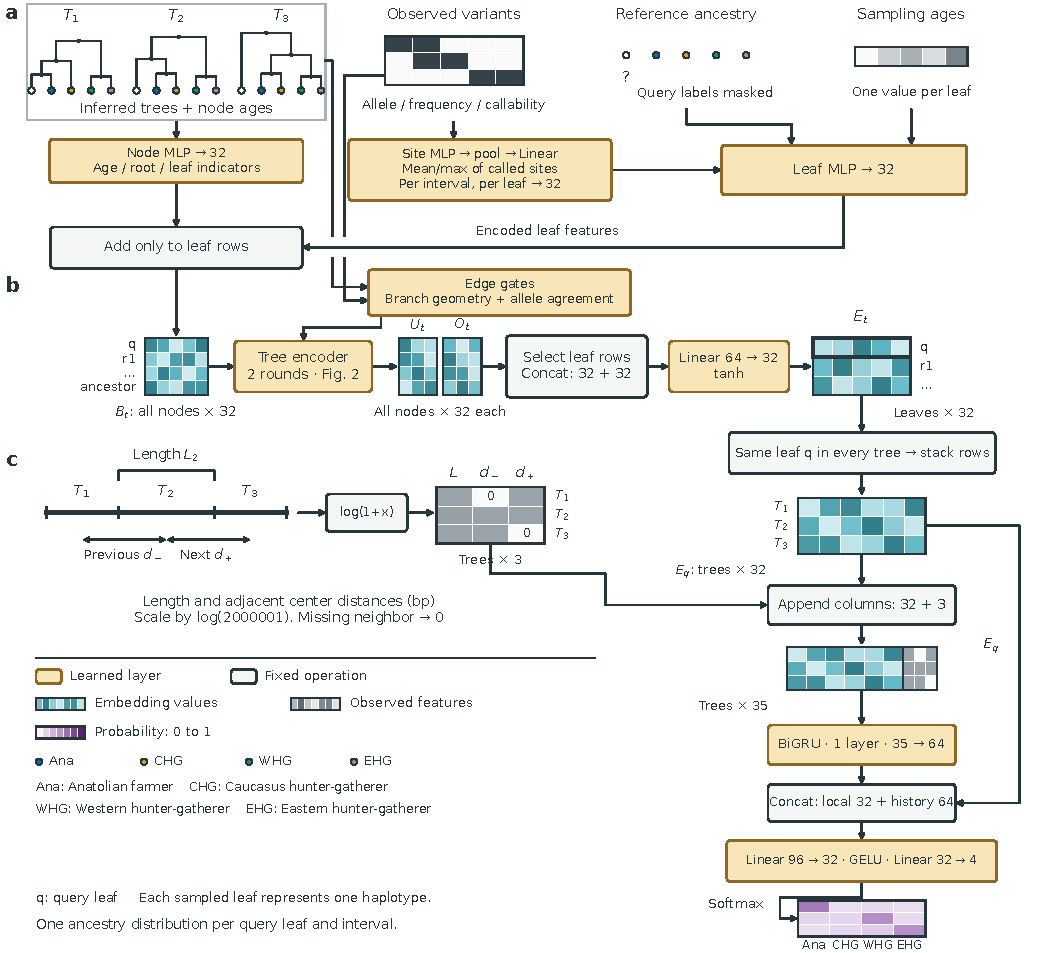
\includegraphics[width=\textwidth]{figures/TreeLoom_architecture.pdf}
\caption{\textbf{a,} Three marginal trees with the same sampled haplotypes. The allele matrix shows one illustrative site per interval. Observed allele frequencies and callability feed the site MLP, then pooling. Reference labels, sampling ages and node features also enter the feature MLPs. Query ancestry is unknown.
\textbf{b,} Vectors at every node show upward states $u$ and outside states $o$, including internal ancestors. Root outside state is zero. Two complete rounds reuse the same node operators, expanded in Figure~\ref{fig:operators}. Memory and structure modify input $b$ before round 2. Concatenating the final states gives one local embedding per haplotype per tree.
\textbf{c,} Interval length $L_t$ and adjacent center distances $d_-,d_+$ form three geometry features, each transformed by $\log(1+x)/\log(2000001)$. Missing neighbors give zero. Geometry joins each local query embedding before the BiGRU and classifier. Feature colors and ancestry probabilities are illustrative, not fitted results. Colors and shapes follow the legend.}
\label{fig:architecture}
\end{figure*}
